\addcontentsline{toc}{chapter}{LAMPIRAN}
\appendix 

\chapter{Kuisioner Identifikasi oleh Ahli}
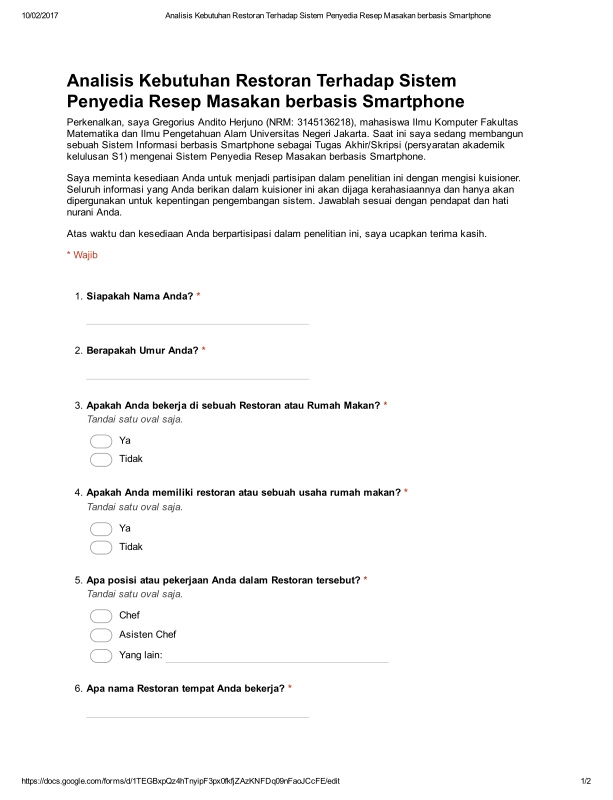
\includegraphics[width=1\textwidth]{pdf/hal_1_ahli}
\includepdf[pages=2-, scale=0.8]{pdf/identifikasi_ahli.pdf}

\chapter{Kuisioner Identifikasi oleh Awam}
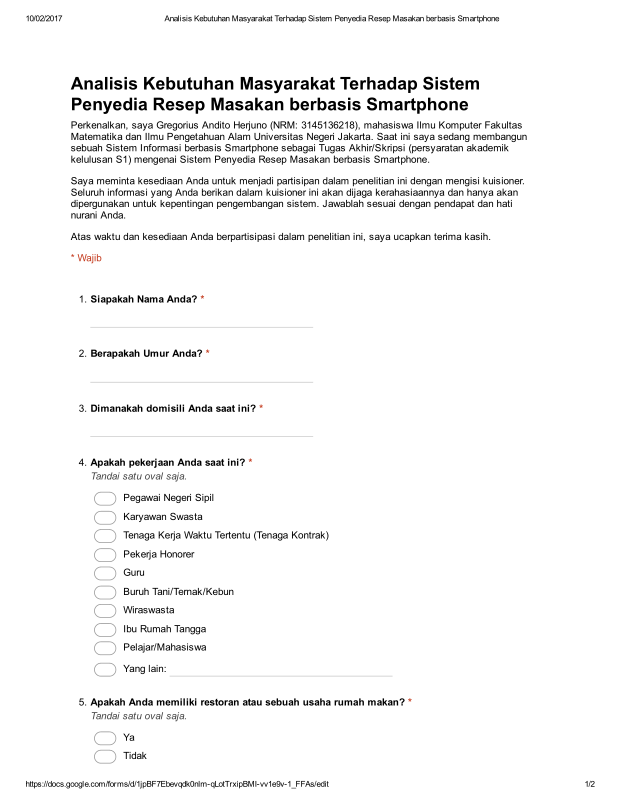
\includegraphics[width=1\textwidth]{pdf/hal_1_masyarakat}
\includepdf[pages=2-, scale=0.8]{pdf/identifikasi_masyarakat.pdf}


\chapter{Sampel API Buatan Penulis Bagian Model}
	\begin{verbatim}
		function get_resep(){
			$obj = $this->db->select('*')
							->get('tb_resep');
			return $obj->result_array();
		}
		
		function get_list_bahan($id_resep){
			$obj = $this->db->select('*')
							->join('tb_list_bahan',
							'tb_list_bahan.id_bahan = tb_bahan.id_bahan')
							->join('tb_satuan',
							'tb_satuan.id_satuan = tb_bahan.id_satuan')
							->where('id_resep',$id_resep)
							->get('tb_bahan');
			return $obj->result_array();
		}
		
		function get_list_cara($id_resep){
			$obj = $this->db->select('*')
						->where('id_resep',$id_resep)
						->get('tb_cara_memasak');
			return $obj->result_array();
		}
		
		function get_search_bahan($query){
			$obj = $this->db->select('*')
							->join('tb_kategori',
							'tb_kategori.id_cat = tb_resep.id_cat')
							->join('tb_bahan',
							'tb_bahan.id_resep = tb_resep.id_resep')
							->join('tb_list_bahan',
							'tb_list_bahan.id_bahan = tb_bahan.id_bahan')
							->like('nama_bahan',$query)
							->get('tb_resep');
			return $obj->result_array();
		}
		
	\end{verbatim}	
\chapter{Sampel API Buatan Penulis Bagian Controller}
	\begin{verbatim}
		function get_resep(){
			$query = $this->Masakyuk_model->get_resep();
			$response = array();
			$cek = $query;
			if($cek > 0){
				$response["resep"]	=array();
				foreach ($query as $row) {
					$data=array();
					$data["id_resep"]		=	$row["id_resep"];
					$data["id_cat"]	=	$row["id_cat"];
					$data["judul"]	=	$row["judul"];
					$data["gambar"]	=	$row["gambar"];
					$data["link_youtube"]	=	$row["link_youtube"];
					$data["rekomendasi"]	=	$row["rekomendasi"];
					array_push($response["resep"], $data);
				}
				$response["success"]	= 1;
				$response["message"]	= "Semua data resep";
				echo json_encode($response);
			} else {
				$response["success"]	= 0;
				$response["message"]	= "Data resep tidak ditemukan";
				echo json_encode($response);
			}
		}
		
		function get_list_bahan_resep(){
			if($this->input->post('id_resep')){
				$id_resep=$this->input->post('id_resep');
			}
			$query = $this->Masakyuk_model->get_list_bahan($id_resep);
			$response = array();
			$cek = $query;
			if($cek > 0){
				$response["bahan"]	=array();
				foreach ($query as $row) {
					$data=array();
					$data["id_resep"]		=	$row["id_resep"];
					$data["id_bahan_utama"]		=	$row["id_bahan_utama"];
					$data["banyaknya"]	=	$row["banyaknya"];
					$data["satuan"]	=	$row["satuan"];
					$data["nama_bahan"]	=	$row["nama_bahan"];
					array_push($response["bahan"], $data);
				}
				$response["success"]	= 1;
				$response["message"]	= "Semua data bahan";
				echo json_encode($response);
			} else {
				$response["success"]	= 0;
				$response["message"]	= "Data bahan tidak ditemukan";
				echo json_encode($response);
			}
		}
		
		function get_list_cara_memasak(){
			if($this->input->post('id_resep')){
				$id_resep=$this->input->post('id_resep');
			}
			$query = $this->Masakyuk_model->get_list_cara($id_resep);
			$response = array();
			$cek = $query;
			if($cek > 0){
				$response["cara"]	=array();
				foreach ($query as $row) {
					$data=array();
					$data["id_resep"]		=	$row["id_resep"];
					$data["id_cara_memasak"]		=	$row["id_cara_memasak"];
					$data["cara"]	=	$row["cara"];
					array_push($response["cara"], $data);
				}
				$response["success"]	= 1;
				$response["message"]	= "Semua cara memasak resep";
				echo json_encode($response);
			} else {
				$response["success"]	= 0;
				$response["message"]	= "Data cara memasak tidak ditemukan";
				echo json_encode($response);
			}
		}
		
		function get_list_hasil_cari(){
			if($this->input->post('query')){
				$query=$this->input->post('query');
			}
			$query = $this->Masakyuk_model->get_search_bahan($query);
			$response = array();
			$cek = $query;
			if($cek > 0){
				$response["resep"]	=array();
				foreach ($query as $row) {
					$data=array();
					$data["id_resep"]		=	$row["id_resep"];
					$data["id_cat"]	=	$row["id_cat"];
					$data["cat"]	=	$row["cat"];
					$data["judul"]	=	$row["judul"];
					$data["gambar"]	=	$row["gambar"];
					$data["link_youtube"]	=	$row["link_youtube"];
					$data["rekomendasi"]	=	$row["rekomendasi"];
					array_push($response["resep"], $data);
				}
				$response["success"]	= 1;
				$response["message"]	= "Semua data resep";
				echo json_encode($response);
			} else {
				$response["success"]	= 0;
				$response["message"]	= "Data resep tidak ditemukan";
				echo json_encode($response);
			}
		}		
	\end{verbatim}	

\chapter{Instrumen Uji Coba Ahli}
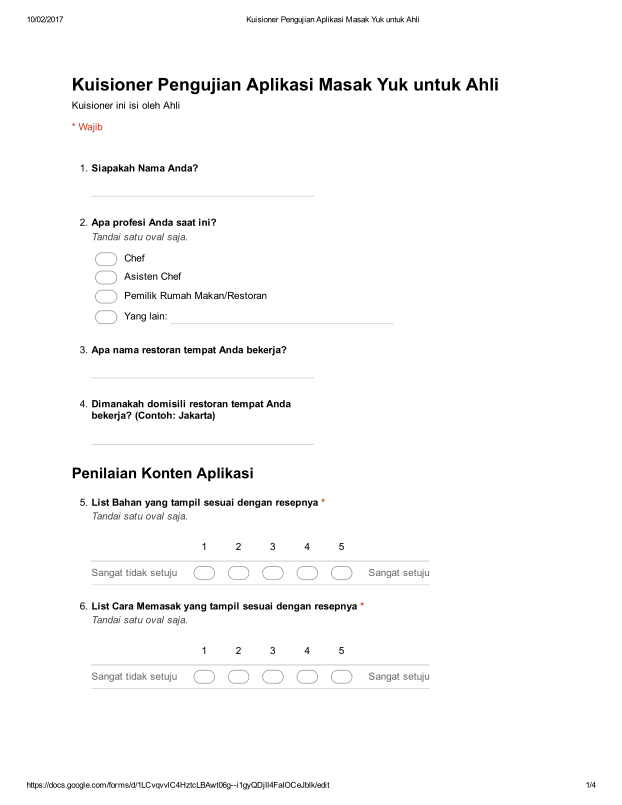
\includegraphics[width=1\textwidth]{pdf/uji_ahli_hal_1}
\includepdf[pages=2-, scale=0.8]{pdf/uji_ahli.pdf}
